\subsection{Wagasci modules}
\subsubsection{Main detector}
The WAGASCI modules are mainly composed of 1280 plastic scintillator bars and a surrounding stainless steel tank as shown in Fig. \ref{fig:3dgrid_wagascimod}.
The total number of channels in one Wagasci module is 1280.
The stainless steel tank is constructed by welding stainless steel plates, is sized as 46$\times$125$\times$125 cm$^{3}$, and weighs 0.5 ton. 
%The plastic scintillator bars form a three-dimensional grid structure with 5$\times$5$\times$2.5 cm$^{3}$ cells. 


One Wagasci module consists of 16 scintillator tracking planes, where each plane is an array of 80 scintillator bars fixed with ABS frames.
The 40 bars, called parallel scintillators, are placed perpendicularly to the beam, and the other 40 bars, called grid scintillators, are placed in parallel to the beam with grid structure in the tracking plane as shown in Fig. \ref{fig:3dgrid_wagascimod}.
Thanks to the 3 D grid-like structure of the scintillator bars, 
the Wagasci module has $4\pi$ angular acceptance for charged particles.

\begin{figure}[tbhp]
  \begin{center}
   \begin{subfigure}{0.48\textwidth}
     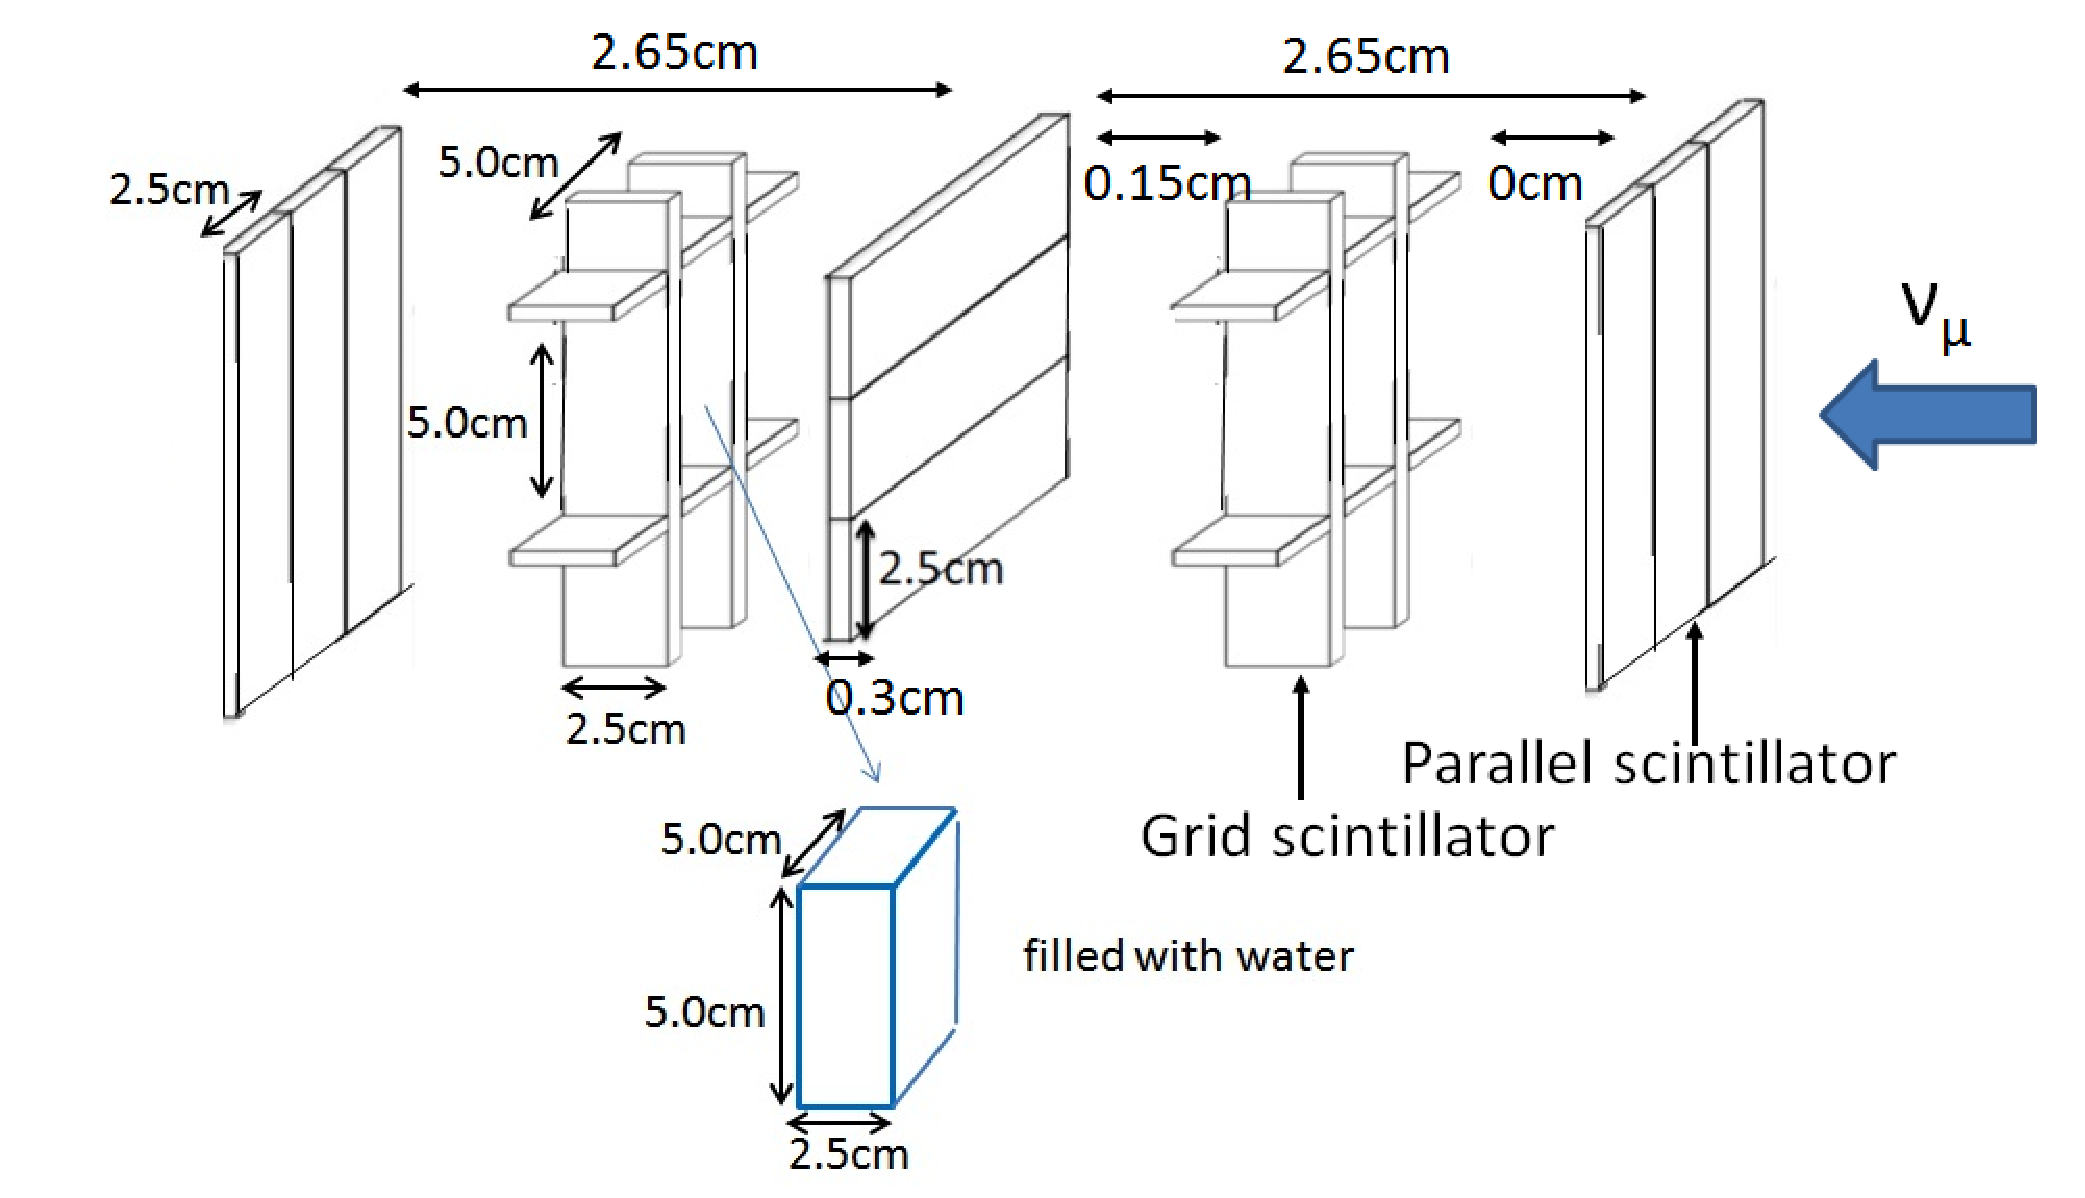
\includegraphics[width=\linewidth]{fig/3d_grid_structure.pdf}
    \end{subfigure}
  \begin{subfigure}{0.48\textwidth}
      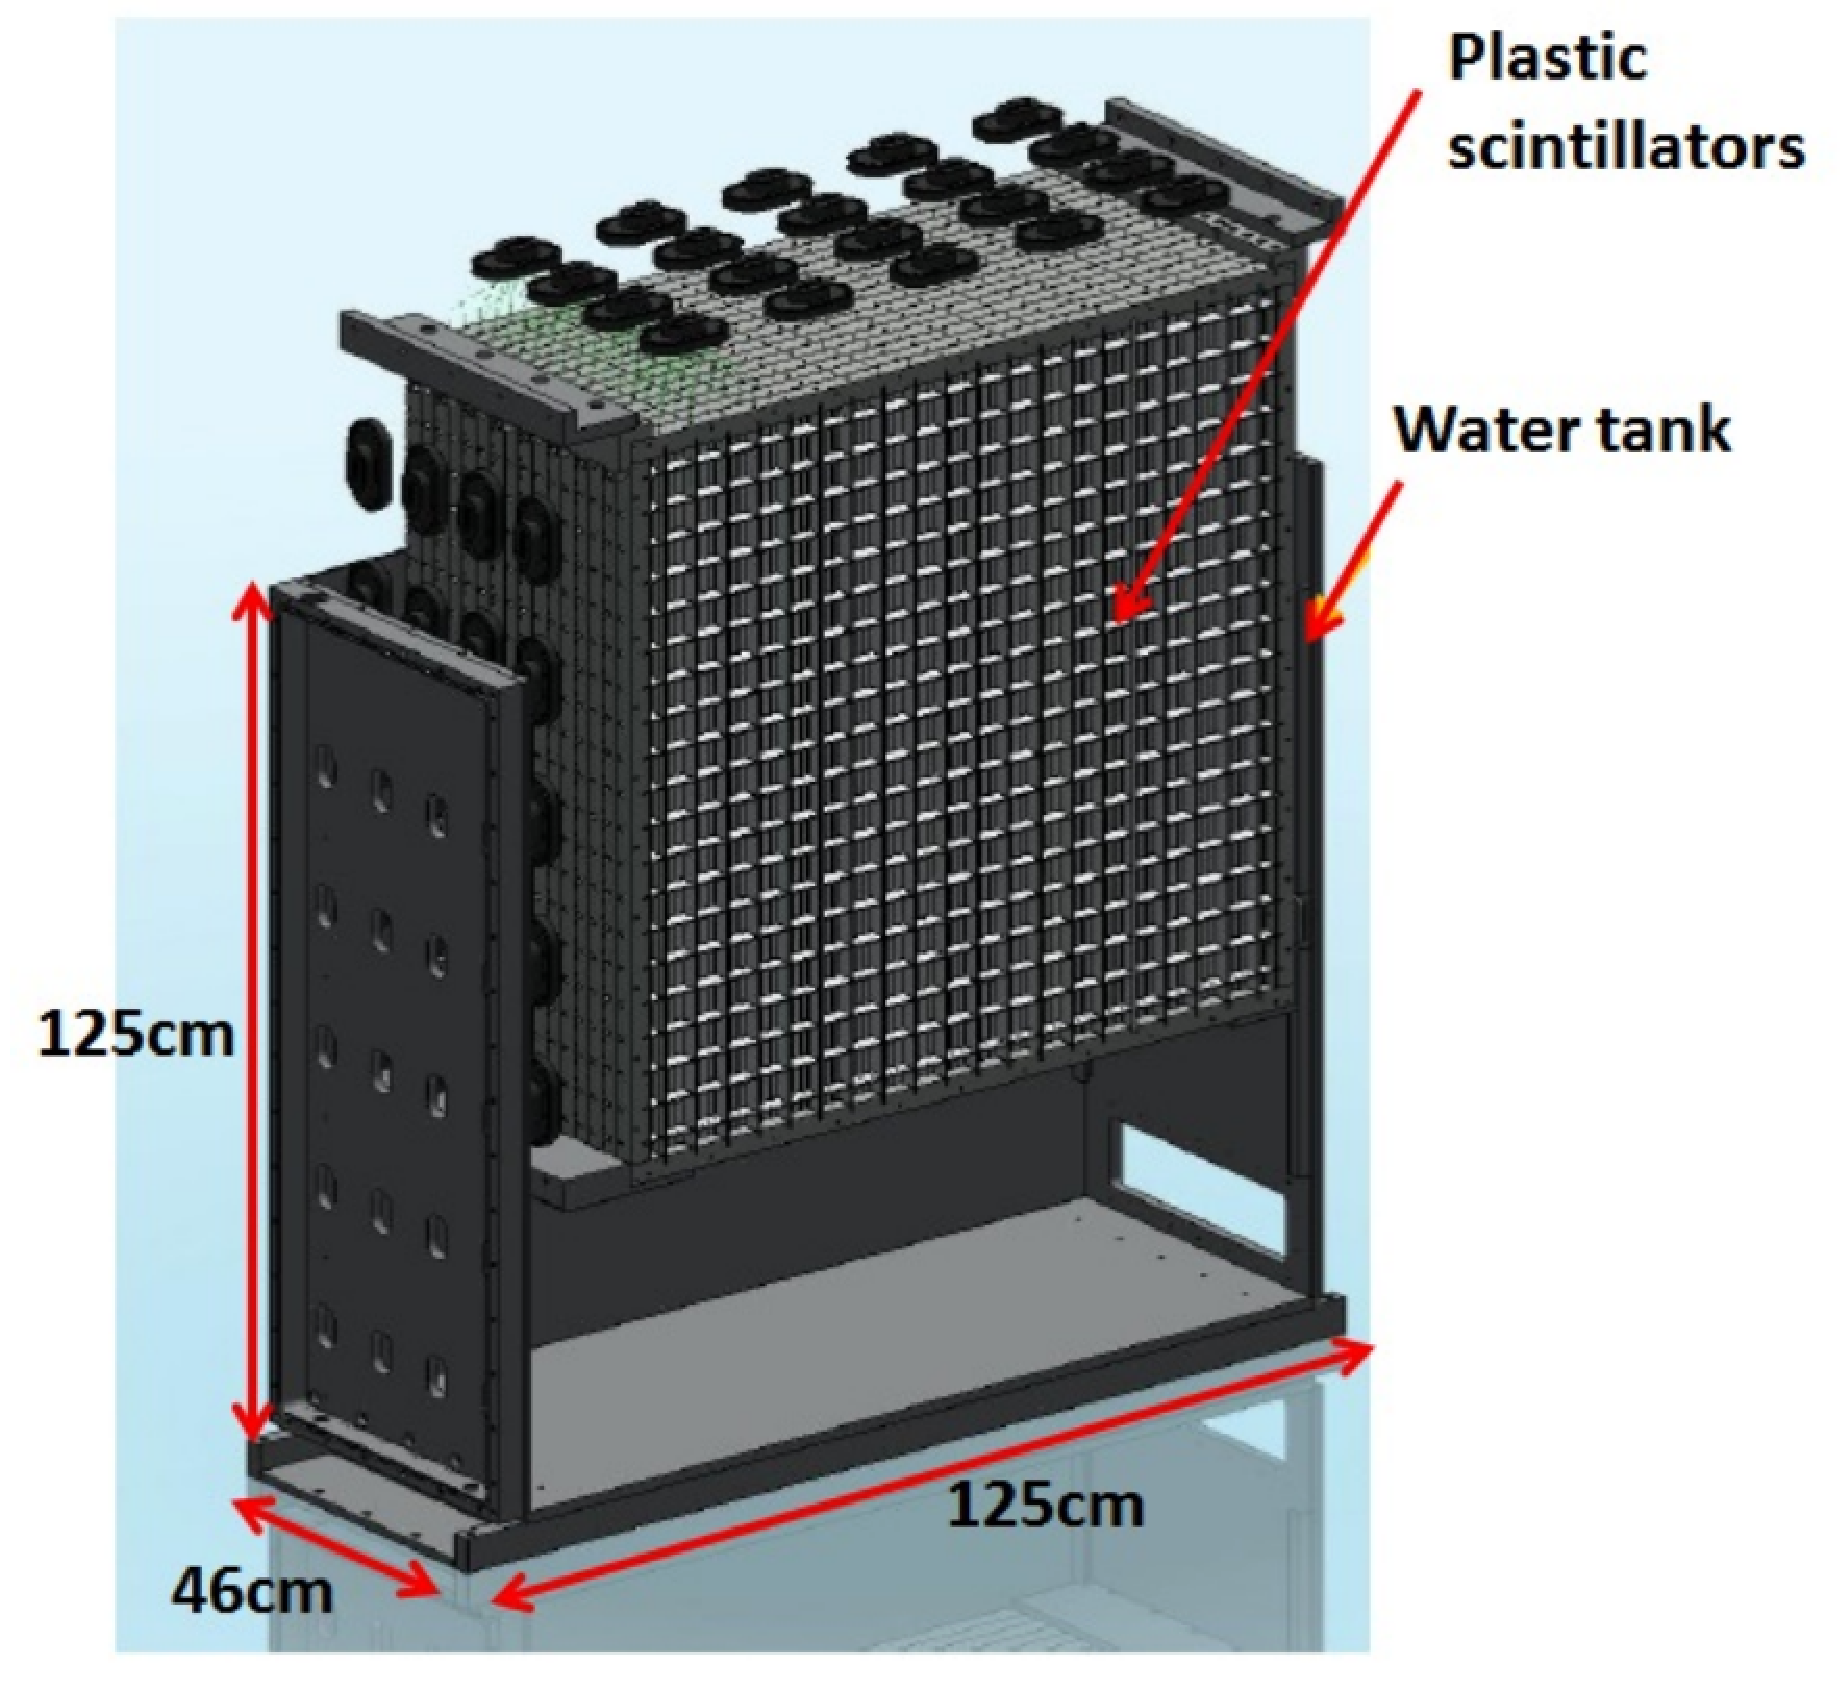
\includegraphics[width=\linewidth]{fig/wagasci_mod.pdf}
    \end{subfigure}    
    \end{center}
  \caption{Schematic views of 3D grid-like structure of plastic scintillator bars (left) and Wagasci module (right).}
\label{fig:3dgrid_wagascimod}
\end{figure}


Thin plastic scintillator bars produced at Fermilab by extrusion method, mainly consists of polystyrene and are surrounded by thin reflector including TiO$^{2}$ (3 mm in thickness) are used for the Wagasci modules to reduce the mass ratio of scintillator bars to water,
because neutrino interactions in the scintillator bars are a background for the cross section measurements on H$_{2}$O.
Each scintillator bar is sized as 1020$\times$25$\times$3 mm$^{3}$ including the reflector part, and 
half of all the scintillator bars have 5-cm-interval slits to form the grid structure (Figure \ref{fig:wagasci_scinti_geometry} ). 

\begin{figure}[tbh]
\begin{center}
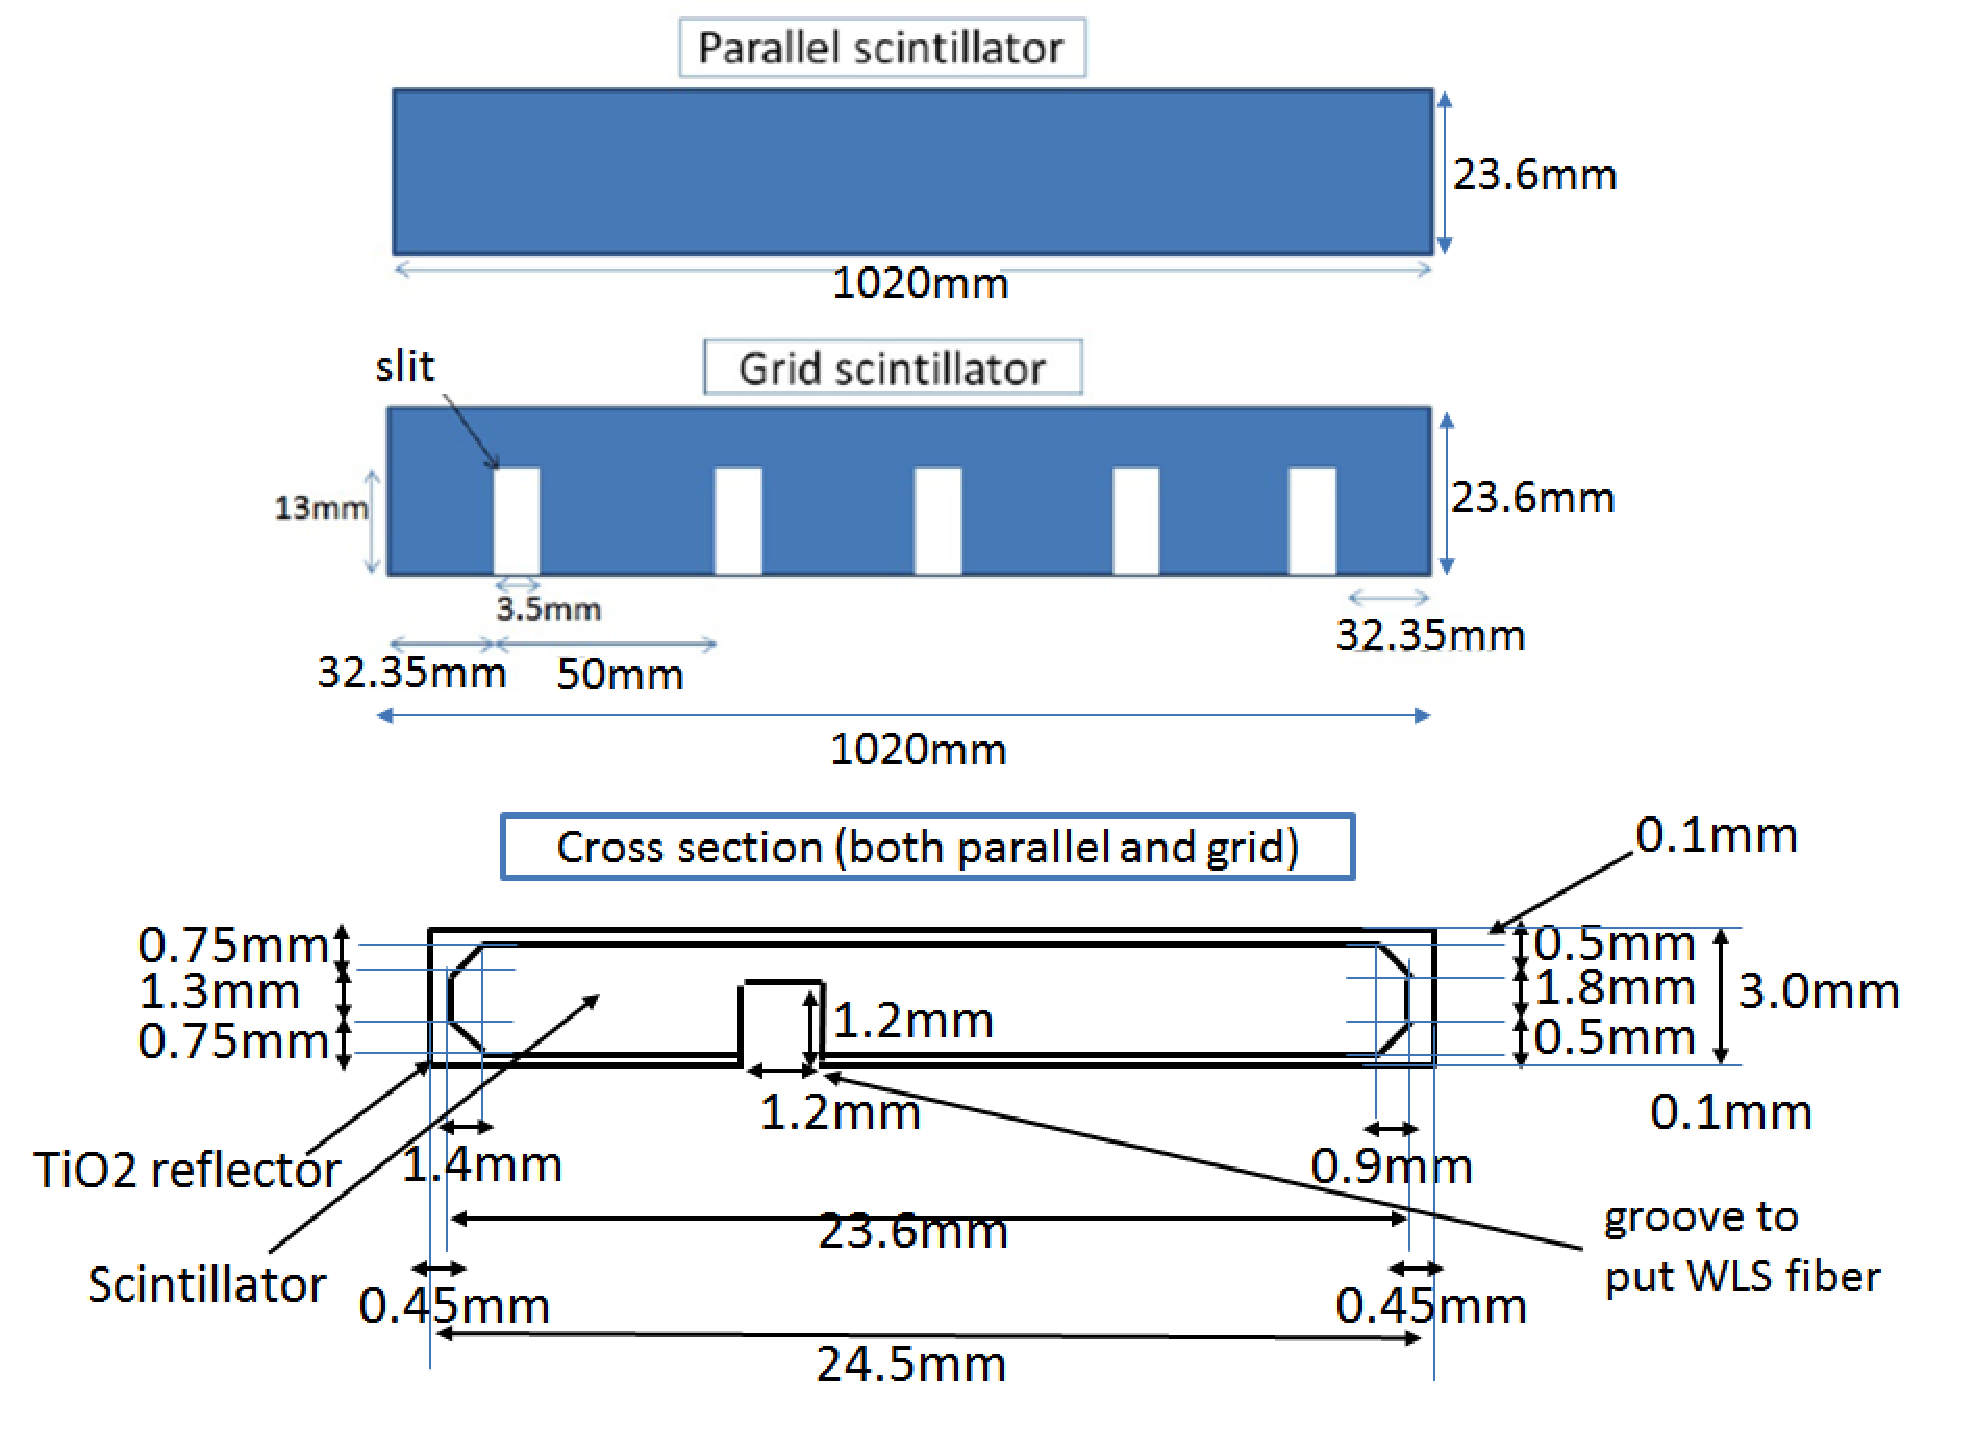
\includegraphics[width=0.8\linewidth]{fig/wagasci_scinti_geometry.pdf}
% 
\includegraphics[width=0.6\linewidth]{fig/tmp.pdf}
\end{center}
\caption{
Geometry of scintillators used for Wagasci modules.
}
\label{fig:wagasci_scinti_geometry}
\end{figure}


We will have two types of the Wagasci modules, a water-in module and a water-out module.
The water-in Wagasci module has water in spaces of the grid structure.
The total water mass serving as neutrino targets in the fiducial volume of the module is 188 kg,
and the mass ratio of scintillator bars to water is 80 \%.
The water-out Wagasci module doesn't have water inside the detector.
The total CH mass serving as neutrino target in the fiducial volume of the module is 47 kg,
and the mass fraction of scintillator bars is 100 \%.


Scintillation light is collected by wave length shifting fibers, Y-11 (non-S type  with a diameter of 1.0 mm produced by Kuraray. A fiber is glued by optical cement in a groove on surface of a scintillator bar, as shown in the Fig 11. 32 fibers are gathered together by a fiber bundle at edge of the module, and lead scintillation light to a 32-channel arrayed MPPC.
Since crosstalk of light yield due to reflection on the inner surface of each cell has been observed, all the scintillator bars are painted black by aqueous color spray, as shown in Fig 12. It is confirmed by measurements with cosmic rays that black painting on the surface of the scintillator bars suppresses this crosstalk so that no significant crosstalk effect is observed within uncertainty.


32-channel arrayed MPPCs, as shown in the Fig 13, are used for this module. The surface of the fiber bundle is polished and directly attached onto the 32-channel arrayed MPPCs. The positions of 32 fibers on the bundle are aligned to fit the channels of MPPCs. The MPPC is a product of Hamamatsu Photonics, S13660(ES1), with suppressed noise rate of $\sim$6 kHz per channel at 0.5 p.e. For each MPPC channel 716 pixels of APD are aligned in a shape of circle.


\subsubsection{Electronics}
As front-end electronics of this detector, a Silicon PM Integrated Read-Out Chip (SPIROC) [3] is adopted.
SPIROC is a 36-channel auto-triggered front-end ASIC, and is produced by OMEGA/ IN2P3. 
It not only contains an analog signal processing part such as amplification and shaping of the waveform, but contains a digital signal processing parts such as auto-trigger and timing measurement.
Charge of MPPC signal is sampled by track-and-hold circuit.
A Front-end electronics board, Active Sensor Unit (ASU), has been developed with the SPIROC2D chip, which is the latest version of SPIROC. 
Each readout board is designed to control a 32-channel arrayed MPPC, and 40 of the ASU boards are aligned on the module surface as shown in Fig 14. 
The data acquisition system used for this detector, including back-end boards, has been developed for prototypes of ultra-granular calorimeters for the International Linear Collider (ILC) [2], and independent of the T2K DAQ system.
To synchronize the DAQ system to J- PARC neutrino beam, pre-beam trigger and beam trigger are sent to the clock control card.
The beam trigger signals are converted from optical signals to NIM signals at NIM module on the B2 floor.
In addition, the information of spill number are delivered with 16-bit ECL level signals, and converted to an Ethernet frame by an FPGA evaluation board to be directly sent to the DAQ PC.
% The event of the WAGASCI module will be off-line matched with those of INGRID placed at the B2 floor and Proton Module by using the spill number information.

\subsubsection{Water system}


